\begin{figure}[h]
    \resizebox{\textwidth}{!}{
    \begin{tikzpicture}[node distance=3cm]
     
        \draw (-80bp,75bp) node[text width=7cm]{\Large \say{A duck is swimming in a pond. A tree is next to the pond.}};
    
        \draw [->] (25bp,75bp) -- (55bp,75bp);
    
        \draw (71.0bp,46.5bp) -- (71.0bp,144.5bp) -- (274.0bp,144.5bp) -- (274.0bp,46.5bp) -- cycle;
        \draw (172.5bp,133.0bp) node {\Large group};
        \draw [->] (133.19bp,92.3bp) .. controls (152.83bp,90.652bp) and (179.94bp,88.375bp)  .. (211.85bp,85.696bp);
        \draw (172.5bp,96.0bp) node {\large IN};
        \draw [->] (133.19bp,31.497bp) .. controls (153.19bp,41.417bp) and (180.93bp,55.183bp)  .. (211.85bp,70.525bp);
        \draw (172.5bp,60.0bp) node {\large NEXT TO};
        \draw (79.0bp,76.5bp) -- (79.0bp,112.5bp) -- (133.0bp,112.5bp) -- (133.0bp,76.5bp) -- cycle;
        \draw (106.0bp,94.5bp) node {\Large duck};
        \draw (212.0bp,65.5bp) -- (212.0bp,101.5bp) -- (266.0bp,101.5bp) -- (266.0bp,65.5bp) -- cycle;
        \draw (239.0bp,83.5bp) node {\Large pond};
        \draw (79.0bp,0.5bp) -- (79.0bp,36.5bp) -- (133.0bp,36.5bp) -- (133.0bp,0.5bp) -- cycle;
        \draw (106.0bp,18.5bp) node {\Large tree};
        
        \draw [->] (285bp,75bp) -- (315bp,75bp);
        
        \draw (425bp, 75bp) node{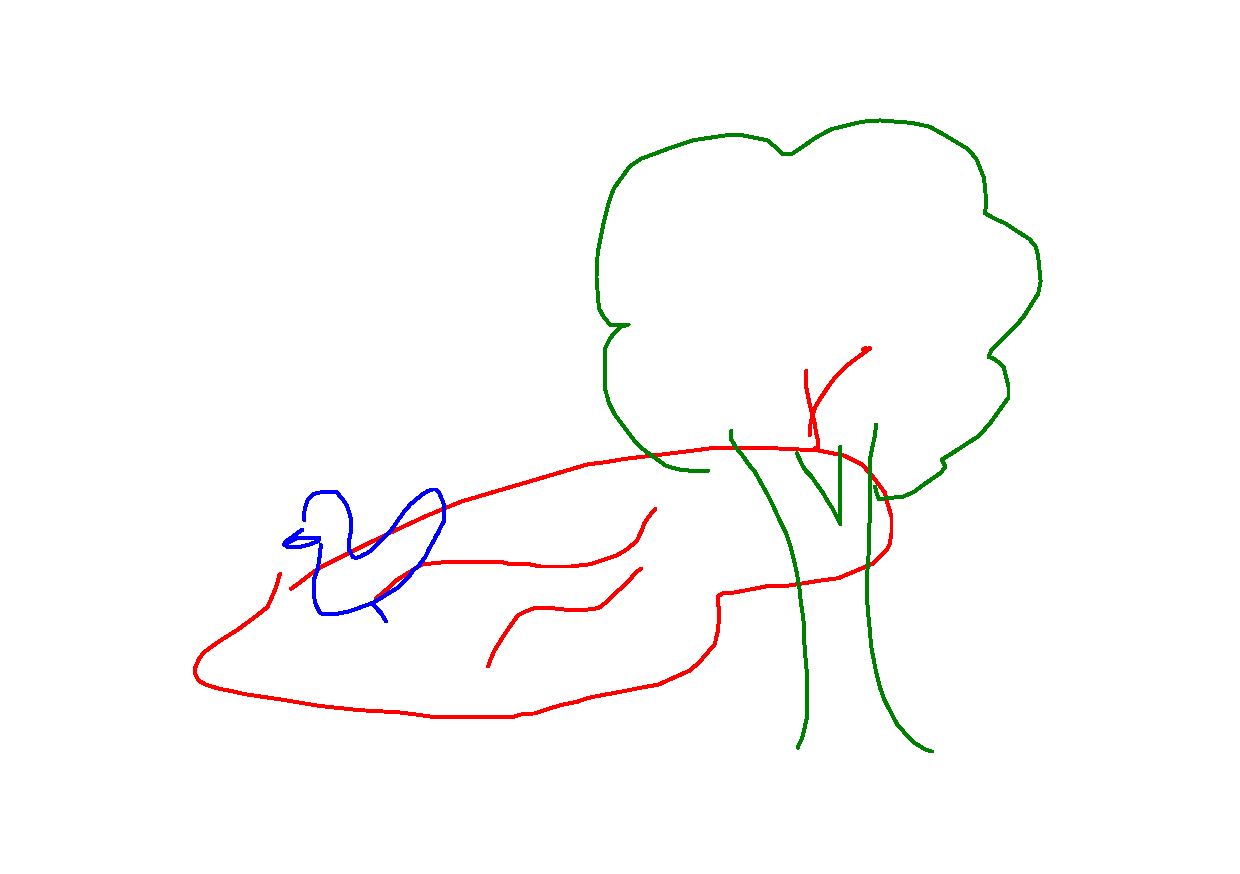
\includegraphics[width=200bp,trim=80 0 80 0,clip]{figures/duck_pond_tree_scene.pdf}};
    
    \end{tikzpicture}
    }
\end{figure}
